\documentclass[tikz,border=8pt]{standalone}
\usepackage{amsmath,amssymb}
\usepackage{tikz}

\begin{document}
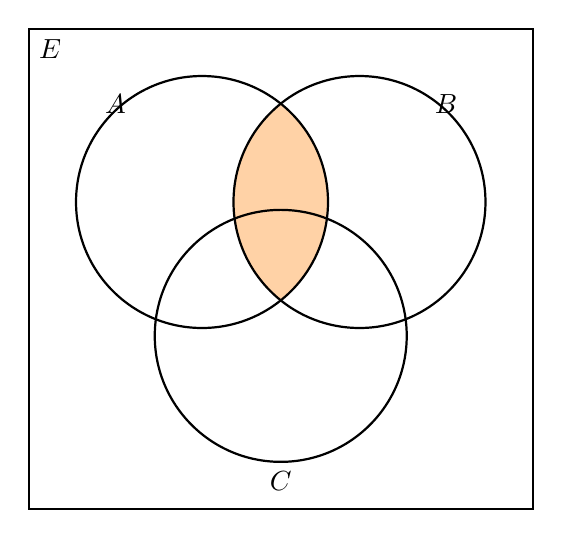
\begin{tikzpicture}[thick]
  \def\A{(0,0) circle (1.6)}
  \def\B{(2,0) circle (1.6)}
  \def\C{(1,-1.7) circle (1.6)}
  \begin{scope}
    \clip \A;
    \fill[orange!35] \B;
  \end{scope}
  \draw \A;
  \draw \B;
  \draw \C;
  \node at (-1.1,1.25) {$A$};
  \node at (3.1,1.25)  {$B$};
  \node at (1,-3.55)   {$C$};
  \draw (-2.2,-3.9) rectangle (4.2,2.2);
  \node[anchor=north west] at (-2.2,2.2) {$E$};
\end{tikzpicture}
\end{document}
